

\subsection{Performance Evaluation}
\label{subsec-perf}


This section evaluates the performance of various aspects of \app including
\sia ($\S$\ref{subsubsec-performance}),
\pia ($\S$\ref{subsubsec-micro})
and the four analysis algorithms ($\S$\ref{subsubsec-compare}).
All the performance evaluations were conducted on a research
cluster with $40$ workstations
equipped with Intel Xeon Quad Core HT 3.7 GHz CPU 
and 16 GB memory.


\subsubsection{\sia: Efficiency v.s. Accuracy}
\label{subsubsec-performance}

We first explore the efficiency/accuracy 
trade-off between the \sia's
two analysis algorithms for analyzing a dependency graph:
the minimal \rg algorithm and 
the failure sampling algorithm (see \S\ref{subsubsec-determine}).
%The former is able to produce a complete
%set of all minimal \rgs but does so within NP-hard complexity.
%The failure sampling algorithm, on the other hand,
%cannot guarantee completeness
%but runs in linear time.
We generated test topologies at three different scales
from a small cloud deployment
to a large deployment as we expect to find in commercial clouds
using the widely accepted three-stage 
fat tree model~\cite{mysore09portland}.
The topologies included typical components within
data centers: servers, Top-of-Rack (ToR) switches,
aggregation switches, and core routers.
Table~\ref{tab-conf} gives the detail of these generated test topologies.
%We run the experiments on a 
%Dell Precision T3600 workstation
%equipped with Intel Xeon E5-1620 v2 Quad Core HT 3.7 GHz CPU 
%and 16 GB memory.


\begin{table}[tbp]
 	\caption{Configurations of our generated data sets.}
	\vspace{-0.2cm}
	\centering{
	\begin{footnotesize} 
	\begin{tabular}{l|r|r|r}
    \hline ~ &  
    Config \#A &
    Config \#B &
    Config \#C \\
    \hline
    \hline
    \# of switch ports & 16 & 24 & 48 \\
    \# of core routers & 64 & 144 & 576 \\
    \# of agg switches & 128 & 288 & 1,152 \\
    \# of ToR switches & 128 & 288 & 1,152 \\
    \# of servers & 1,024 & 3,456 & 27,648 \\ 
    \hline
    \hline
    \footnotesize{Total \# of devices} & 1,360 & 4,200 & 30,528 \\
    \hline
  \end{tabular}
	\end{footnotesize}
  }
  \label{tab-conf}
\end{table}


We compared the run-time of the accurate but NP-hard minimal \rg algorithm
to that of a failure sampling algorithm with different sampling rounds ($10^3$ to $10^7$).
Figure~\ref{fig-simulation} presents the result.
%With the minimal \rg algorithm as a baseline,
%we evaluated accuracy versus run-times
%for the failure sampling algorithm.
It shows that the failure sampling algorithm
runs much more efficiently with a reasonably high accuracy.
In configuration \#B, for example, the failure sampling algorithm
detects 92\% of all the minimal \rgs using about 90 minutes with $10^6$ samplings,
in comparison to 1046 minutes for the minimal \rg algorithm.
%In the last two configurations, 
%the failure sampling algorithm (with $10^6$ rounds)
%balances performance and accuracy better than the ones (with $10^5$ 
%and $10^7$ rounds) and minimal cut set algorithm.
%; thus, we suggest that
%the failure sampling algorithm with $10^6$ rounds is the most
%suitable to auditing large scale clouds.


% 5k^2/4 k-port switches support k^3/4 hosts for fat tree model


\subsubsection{\small{\pia: Microbenchmarks and System Overheads}}
\label{subsubsec-micro}


For \pia evaluation,
we implemented another private set intersection 
cardinality protocol, Kissner and Song (KS)~\cite{kissner05privacy},
in our prototype used to compare with \pso.


For any privacy-preserving system, 
cryptographic operations tend to be 
the major computational bottleneck.
Thus, we evaluated the overhead of \pia 
through comparing \pso with KS.
All the cryptographic primitives of \pso
include hash, commutative encryptions and shuffle.
For KS, it uses homomorphic encryption and decryption, 
calculations on encrypted polynomial and shuffle.
In the microbenchmark evaluation,
we generated three data sets 
containing between $1,000$ and $100,000$ elements each.
We measured both the run-time and network traffic
using both \pso and KS.
We compute run-time as the total time in seconds to perform the evaluation
and measure the network traffic in terms of the total number of bytes
transferred among participants in the system.


Figure~\ref{subfig-bench-net} and \ref{subfig-bench-com} show
microbenchmarks for bandwidth overhead 
and computational overhead, respectively.
In Figure~\ref{subfig-bench-com},
the time of \pso increases almost linearly with the
size of data sets, while the computational overhead of
KS increases polynomially with the size of data sets.
As shown in Figure~\ref{subfig-bench-net},
both protocols transmit traffic proportional
to the data set sizes.


\begin{figure*}[tbp] \centering
\subfloat[Bandwidth overhead.]{
    \label{subfig-bench-net}
    \begin{minipage}[t]{0.42\textwidth}
    \centering
        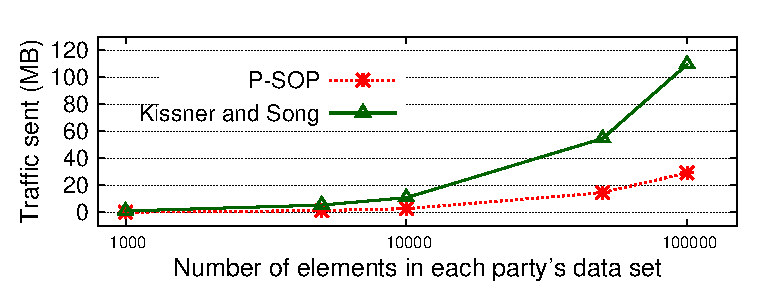
\includegraphics[width=1\textwidth]{figs/bench-net.eps}
    \end{minipage}
}\hfill \subfloat[Computational overhead.]{
    \label{subfig-bench-com}
    \begin{minipage}[t]{0.42\textwidth}
    \centering
        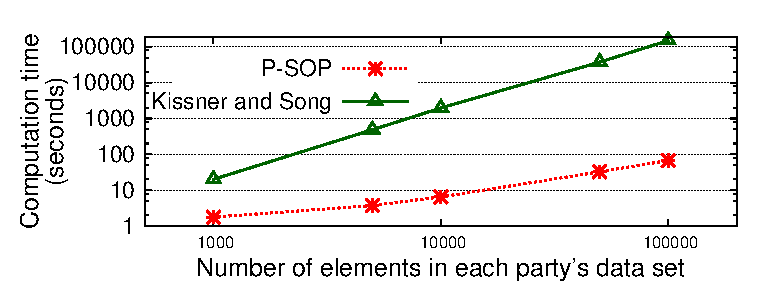
\includegraphics[width=1\textwidth]{figs/bench-com.eps}
    \end{minipage}
}\\\vspace{-0.34cm}
\subfloat[Bandwidth overhead.]{
    \label{subfig-net}
    \begin{minipage}[t]{0.42\textwidth}
    \centering
        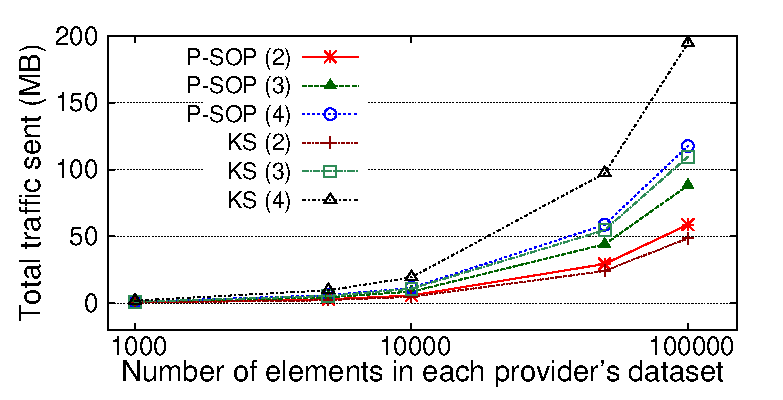
\includegraphics[width=1\textwidth]{figs/net.eps}
    \end{minipage}
}\hfill \subfloat[Computational overhead.]{
    \label{subfig-com}
    \begin{minipage}[t]{0.42\textwidth}
    \centering
        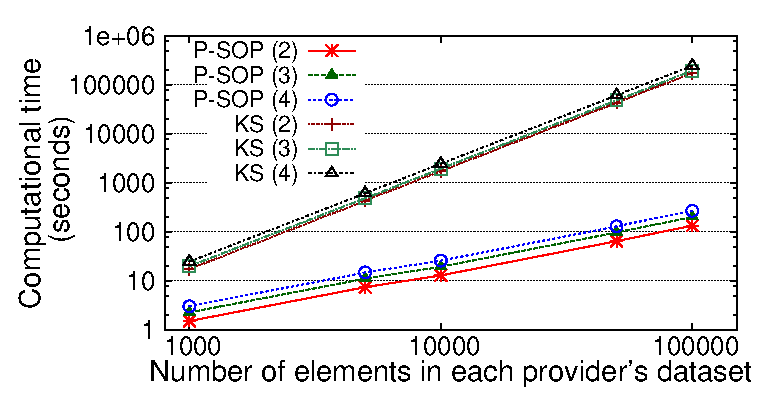
\includegraphics[width=1\textwidth]{figs/com.eps}
    \end{minipage}
}\vspace{-0.3cm}
\caption{Microbenchmarks and system overhead.  
The public key crypto schemes use a 1024-bit key.} 
\label{fig-bench}
\end{figure*}


We now compare \pso with KS in terms of
their computational and bandwidth overheads
at each cloud provider, 
which is the bottleneck of the whole system.
In this evaluation, there are $k$ providers (replicas) ran
both \pso and KS protocols
with $n$ elements in each of their data sets.
We vary $n$ between $1,000$ and $100,000$,
and set $k$ to $2$, $3$ and $4$ respectively.
The computational and bandwidth overhead
are the same as the definitions
of measuring microbenchmarks.\abbr{}{, \ie,
all the time required by cryptographic operations
and the size of encrypted messages sent.}
Figure~\ref{subfig-net} and Figure~\ref{subfig-com}
show each provider's bandwidth and
computational overhead, respectively.
For computational overhead, \pso is much efficient than KS.
\abbr{}{Moreover, in a three redundancy deployment, 
an alternative service provider owning 
a local data set with $100,000$ elements can finish all
the computation operations with about $200$ seconds,
if the provider is using \pso.
Regarding bandwidth, we concede KS protocol
is less than \pso in the two redundancy deployment case.
However, \pso is more efficient than KS
in other two cases.}

\com{
\begin{figure}[tbp] \centering
\subfloat[Bandwidth overhead.]{
    \label{subfig-net}
    \begin{minipage}[t]{0.42\textwidth}
    \centering
        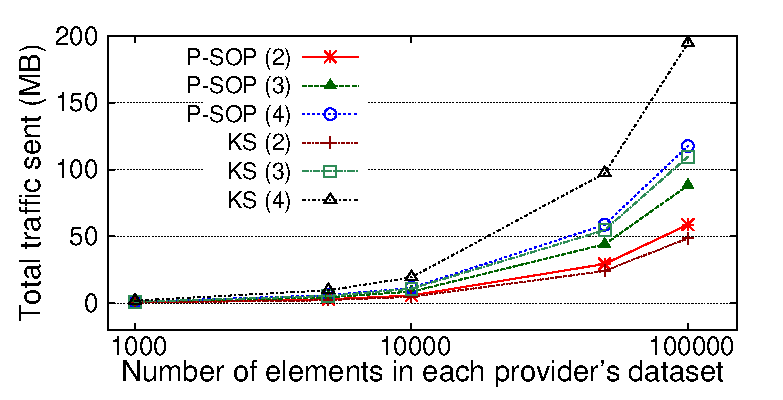
\includegraphics[width=1\textwidth]{figs/net.eps}
    \end{minipage}
}\\ \subfloat[Computational overhead.]{
    \label{subfig-com}
    \begin{minipage}[t]{0.42\textwidth}
    \centering
        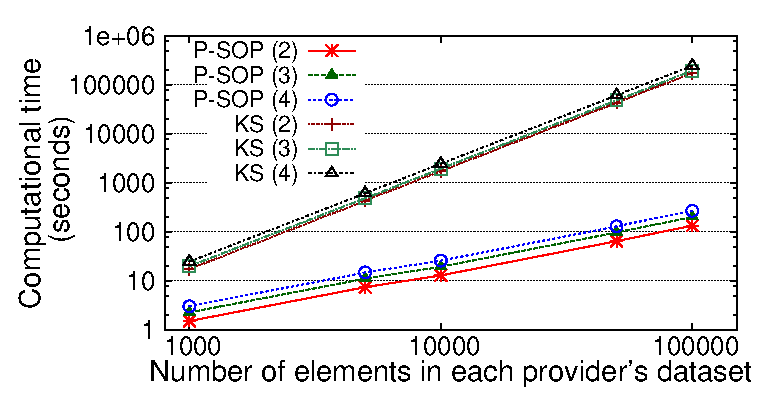
\includegraphics[width=1\textwidth]{figs/com.eps}
    \end{minipage}
}\caption{System overheads.  The public key crypto
schemes use a 1024-bit key.  \pso (n) and Kissner and Song (n)
denotes that $n$ parties perform the protocol 
respectively.} \label{fig-overhead}
\end{figure}
}

%To illustrate \pia's performance gains and scalability, 



\subsubsection{Comparing Four Analysis Algorithms}
\label{subsubsec-compare}


We now compare the performances of four analysis algorithms: 
failure sampling algorithm with ($10^6$) rounds,
minimal \rg algorithm, \pso and KS.
We construct a scenario where there are $n$ cloud providers.
Each of them maintains a local data set
at component-set level of detail containing $10,000$ items.
We perform four algorithms on this scenario
and measure run-time by changing $n=5, 10, 15$ and $20$.
Figure~\ref{subfig-2rep} and Figure~\ref{subfig-3rep}
present run-time of quantifying independence of all the potential 
two and three way replications.

\begin{figure}[tbp] \centering
\subfloat[Analyzing all the potential two-way replications.]{
    \label{subfig-2rep}
    \begin{minipage}[t]{0.4\textwidth}
    \centering
        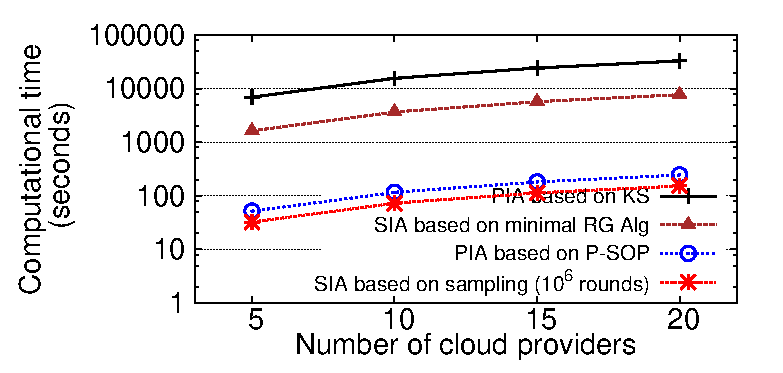
\includegraphics[width=1\textwidth]{figs/2-10000-way.eps}
    \end{minipage}
}\\\vspace{-0.3cm}\subfloat[Analyzing all the potential three-way replications.]{
    \label{subfig-3rep}
    \begin{minipage}[t]{0.4\textwidth}
    \centering
        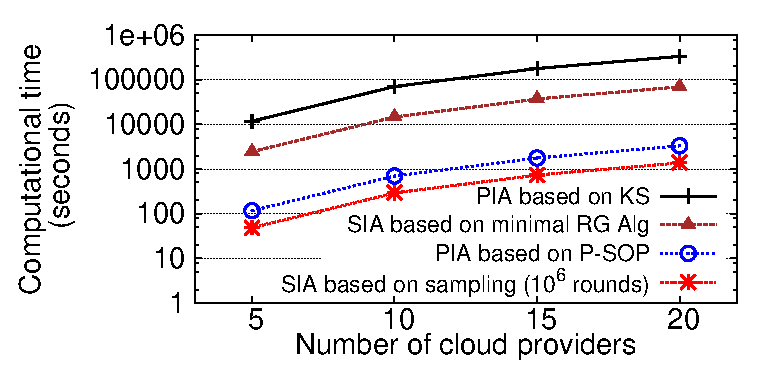
\includegraphics[width=1\textwidth]{figs/3-10000-way.eps}
    \end{minipage}
}\vspace{-0.3cm}
\caption{Quantifying independence of all the potential 
two and three way replications.  Each
provider's data has $10,000$ items of dependency information.} 
\label{fig-compare}
\end{figure}


